% Adapt ME 537 HW04 P1(b) and HW03 frame-chain concepts without DH.
% Shared layout adapted from the instructor's ME 537 homework sources.
\documentclass[12pt,letterpaper]{article}
\usepackage{mathptmx}
\usepackage[T1]{fontenc}
\usepackage{xcolor,amsmath,amssymb,xurl,listings,enumitem,tikz}
\textwidth=6.5in
\textheight=9in
\oddsidemargin=0in
\evensidemargin=0in
\topmargin=0in
\headheight=0in
\headsep=0in
\parskip=0.08in
\parindent=0in
\setlist[enumerate]{itemsep=0.04in,topsep=0.04in}
\lstset{basicstyle=\ttfamily\footnotesize,breaklines=true,columns=fullflexible,
keepspaces=true,showstringspaces=false,aboveskip=0.04in,belowskip=0.04in}
\newcommand{\R}[2]{{}^{#1}\!R_{#2}}
\newcommand{\T}[2]{{}^{#1}\!T_{#2}}
\newcommand{\courseheader}[2]{%
\setlength{\fboxrule}{2pt}\setlength{\fboxsep}{2mm}%
\fcolorbox{black}{white}{\parbox{\dimexpr\linewidth-2\fboxsep-2\fboxrule\relax}{\centering\textbf{Introduction to Robotics Homework \##1 -- Draft}}}\par
\textbf{#2}\par}
\newcommand{\conventions}{Use right-handed rotations, column vectors, radians,
and meters. $\R{A}{B}$ maps coordinates from frame $B$ into frame $A$;
$\T{A}{B}$ also includes the origin of $B$ expressed in $A$.}
\newcommand{\submission}{\textbf{Submit:} labeled hand derivations and sketches,
your changed Python source files, the requested numerical/visual evidence,
and an AI-use statement (including ``none'' if applicable). Show your reasoning
before using code to check hand calculations. Public checks are intentionally
limited. The instructor supplies the deadline and submission destination.}

\begin{document}
\courseheader{4}{General forward kinematics with explicit joints}
\textbf{Schedule:} week 4, approximately one week. Build on HW02--HW03.
\conventions

\begin{enumerate}
\item \textbf{Read the small arm model.}
The supplied \texttt{Joint} class stores a local axis, a motion type, and
fixed \texttt{origin}/\texttt{tip} transforms. It provides
\texttt{joint.transform(q)}. The supplied \texttt{SerialArm} constructor
stores the joint list, base placement, and tool offset.
\begin{enumerate}
\item Explain \texttt{self.joints}, \texttt{self.n}, and one call to
\texttt{joint.transform(q[i])}. Which values describe geometry, and which
change when the arm moves? Joint displacements use radians or meters.
\item For the supplied \texttt{spatial\_arm()} in \path{homework/models.py},
write its three link transforms from these physical descriptions:
\begin{center}
\begin{tabular}{cll}
Joint & Motion axis in its local joint frame & Following fixed offset \\
\hline
1 & Z rotation $q_1$ & $h=0.2$ m along local Z \\
2 & Y rotation $q_2$ & $L_1=0.4$ m along local X \\
3 & Y rotation $q_3$ & $L_2=0.3$ m along local X
\end{tabular}
\end{center}
The joint origins have no additional offset. Apply each joint motion before
its following offset. Frames are numbered 0 through 3. At zero displacement:
\begin{center}
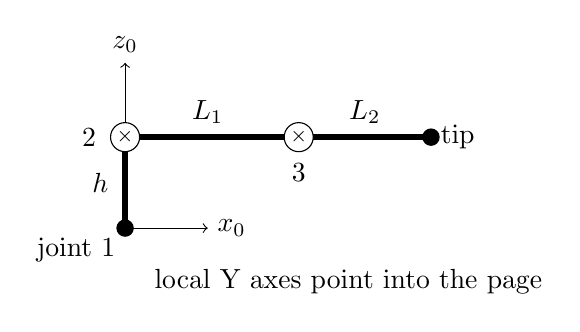
\begin{tikzpicture}[scale=1.05]
\draw[->] (0,0)--(1,0) node[right]{$x_0$};
\draw[->] (0,0)--(0,2.0) node[above]{$z_0$};
\draw[line width=2pt] (0,0)--(0,1.1)--(2.1,1.1)--(3.7,1.1);
\fill (0,0) circle (3pt) node[below left]{joint 1};
\draw[fill=white] (0,1.1) circle (5pt) node[left=7pt]{2};
\draw[fill=white] (2.1,1.1) circle (5pt) node[below=6pt]{3};
\node at (0,1.1){\scriptsize$\times$};\node at (2.1,1.1){\scriptsize$\times$};
\fill (3.7,1.1) circle (3pt) node[right]{tip};
\node at (-0.3,0.55){$h$};\node at (1.0,1.4){$L_1$};\node at (2.9,1.4){$L_2$};
\node at (2.7,-0.65){local Y axes point into the page};
\end{tikzpicture}
\end{center}
The diagram is a side view at $q=0$, not a restriction to planar motion.
\end{enumerate}

\item \textbf{Derive the spatial FK by hand.}
\begin{enumerate}
\item Compose the three transforms to find $\T{0}{3}(q)$.
Give its rotation and position blocks. You may abbreviate
$c_1=\cos q_1$ and $c_{23}=\cos(q_2+q_3)$, with analogous sine notation.
\item Evaluate the full matrix at $q=[0,0,0]$ and
$q=[\pi/2,0,-\pi/2]$. Sketch the arm and final frame in both poses.
Then use code to check your derivation.
\end{enumerate}
\end{enumerate}

\newpage
\begin{enumerate}[start=3]
\item \textbf{Implement the chain product.}
In \path{src/intro_robotics/kinematics.py}, complete \texttt{SerialArm.fk}.
The constructor and checks are provided; do not implement DH or alter
\texttt{Joint.motion}. Your task is the matrix composition.
\begin{enumerate}
\item Use the supplied \texttt{start}/\texttt{end} indices. A scalar
\texttt{index} selects an end frame; a pair selects \texttt{(start,end)}.
The loop composes the joints from \texttt{start} up to, but excluding,
\texttt{end}. An empty chain has an identity transform.
\item Apply the optional base transform only when the chain starts at 0,
and the optional tool transform only when it ends at \texttt{self.n}.
The default result is relative to frame 0, excluding both optional transforms.
\item Run \texttt{python -m homework.hw04.hw04\_fk}. Check one relative
subchain, such as \texttt{index=(1,3)}, against your own matrix product.
Explain its input and output frames.
\end{enumerate}

\item \textbf{Check base/tool offsets and a translating joint.}
\begin{enumerate}
\item At the second pose from problem 2, add a tool offset of 0.1 m along
frame 3's Z axis. Place frame 0 in a world using rotation
$\operatorname{Rot}_z(\pi/2)$ and translation $[1,0.2,0]^T$ meters.
Calculate the tool position in the world by hand. Compare with
\texttt{fk(q, base=True, tip=True)} on the corresponding arm.
\item Inspect the supplied \texttt{slider\_arm()}. Its first joint rotates
about Z; its second slides along its local X. With the first joint held at
$\pi/2$, which world direction should a positive slider displacement move
the tip? Predict the tip position at slider displacement 0.1 m, then check it.
You do not need to change the FK method for this different joint type.
\end{enumerate}

\end{enumerate}

\newpage
\begin{enumerate}[start=5]
\item \textbf{Describe the arm in URDF and compare TF with your FK.}
ROS describes robots in URDF files. A URDF \emph{joint} places its child
link's frame in its parent link's frame: first its fixed \texttt{origin}
(translation \texttt{xyz}, then rotation \texttt{rpy}), then its motion about
\texttt{axis}. The starter \path{homework/hw04/arm.urdf} supplies every link
and its visual, \texttt{world\_joint} (problem 4(a)'s base placement), and
\texttt{joint1} as an example.
\begin{enumerate}
\item Add \texttt{joint2} and \texttt{joint3} (revolute) and
\texttt{flange\_joint} and \texttt{tool\_joint} (fixed), so that
\texttt{arm\_flange} is FK frame 3 and \texttt{arm\_tool} is problem 4(a)'s
tool. URDF has no separate tip offset: explain where each \texttt{Joint}'s
\texttt{tip} from problem 1 appears in your URDF.
\item Show the arm and compare, using two container shells:
\begin{lstlisting}
ros2 launch homework/hw04/view_arm.launch.py
python3 -m homework.hw04.compare_tf
\end{lstlisting}
Set the sliders to problem 2's second pose. The script prints the tool
position from TF (computed by ROS from your URDF) beside
\texttt{fk(q, base=True, tip=True)}; both should match your problem 4(a)
hand result. Save a screenshot of RViz and the printed comparison, then try
one pose of your own.
\item A URDF \texttt{rpy="r p y"} means
$R=\operatorname{Rot}_z(y)\operatorname{Rot}_y(p)\operatorname{Rot}_x(r)$.
Read it in the current frame, as in HW02 problem 2(a): yaw about Z, then
pitch about the new Y, then roll about the new X.
Write \texttt{world\_joint}'s rotation as a matrix and compare it with
problem 4(a). The link visuals use \texttt{rpy="0 1.5708 0"} to lay a
cylinder (whose length runs along its local Z) along X; show why with
$\operatorname{Rot}_y$.
\item TF frame \texttt{arm\_link3} sits at joint 3. Which FK frame has the
same origin, and why do their orientations differ when $q_3\neq 0$?
\item The launch file starts three nodes: the slider window
(\texttt{joint\_state\_publisher\_gui}), \texttt{robot\_state\_publisher},
and RViz. Explain this chain in your own words:
\begin{center}\small
sliders $\longrightarrow$
\texttt{/joint\_states} $\longrightarrow$
\texttt{robot\_state\_publisher} $\longrightarrow$
\texttt{/tf} $\longrightarrow$ RViz.
\end{center}
What does each topic carry, and what does \texttt{robot\_state\_publisher}
need from your URDF to turn joint angles into \texttt{/tf}? In HW01, your
own node took the sliders' place in this chain; why did RViz still show the
robot moving?
\end{enumerate}
The pyqtgraph slider viewer (\texttt{python -m homework.hw04.play\_arm})
remains available for exploring your FK.
\end{enumerate}

\textbf{What to understand:} FK is composition of physical joint/link
transforms. The same short loop handles spatial and prismatic mechanisms,
and a URDF stores the same fixed offsets and joint axes for ROS. Neither
requires a DH table or orientation-conversion functions.

\submission
\end{document}
